\documentclass[../Dissertation.tex]{subfiles}

\begin{document}
\section{Evaluation of experimental design}
\textbf{\color{red}
\begin{itemize}
    \item clear result presentation
    \item explain problems and difficulties
    \item demonstrate understanding of results
    \item discuss further work
\end{itemize}
}
\subsection{Pipeline Development challenges}


In order to accomplish Objective~\hyperref[obj:VerifyComp]{O0} before building the pipeline we manually ran each discrete part of the system (Distiller, and OpenVino). 
This immediately highlighted a critical issue; Distiller by default only zeros out the weights when pruning, it doesn't actually remove them from the model so unless a special flag is used with Distiller called `thinnify' there is no measurable benefit to pruning, this issue is exacerbated by the fact that not all pruning algorithms have been implemented to work with `thinnify' and there is little to no documentation on which are compatible. 
A trial and error approach was taken to find pruning algorithms with a working implementation of `thinnify', we systematically tested each of the pruning algorithms that used coarse grained pruning and eventually identified the algorithm described in Section~\ref{sec:FilterPruningAlgo} as fully functional with `thinnify'.

Once we had a verifiable improvement in latency from the `no-pruning' baseline described in Section~\ref{sec:baselineData}, we proceeded to develop the pipeline according to Objective~\hyperref[obj:BuildPipeline]{O2}.
Setting up the benchmarking and model queue was very straight forward, for the queue we simply pulled down a docker image of Redis and ran it.
The OpenVino benchmarking tool was very easy to integrate into the pipeline, we simply cleared and then wrote the relevant arguments to \texttt{sys.argv} (pythons array of command line arguments), called the main method of the benchmarking tool inside OpenVino, and captured the output.

Development of the Pruning \& retraining part of the pipeline was considerably more challenging, we encountered a couple of issues that we resolved on our own \href{https://github.com/friedforfun/distiller?organization=friedforfun&organization=friedforfun}{\underline{\color{blue}fork of Distiller}}; the namespace of the python standard library \texttt{parser} module is shadowed by distiller which caused issues with our implementation, we also resolved an issue where Distiller would not correctly construct the path to model checkpoints once they were thinnified.
We had persistent issues capturing the output of Distiller (and therefore the location of the models and checkpoint files) because it uses a custom logging solution that overwrites any redirects from the standard output, we resorted to using a file watcher to detect the location of checkpoint files and exported models.
 


\subsection{Hardware and Software}
Both the pruning and benchmarking software runs on Ubuntu 20.04, we used various hardware configurations for the pruning and retraining agents. 
The benchmarking system was fixed for the duration of the project; a KVM virtual machine, 4 cores/8 threads from a Ryzen 3960X, 8Gb RAM, and the Intel Neural Compute Stick was plugged into a USB controller that was passed through to the VM.
Originally the benchmarking system was combined with the pruning system, however due to library and python version compatibility issues we had to run OpenVino and Distiller independently this naturally led us to split the system across multiple machines with Redis as a message queue.


\noindent\textbf{Pruning \& retraining software | library specification}
\begin{itemize}
    \item Python 3.7.10
    \item Distiller | A python package for neural network compression research
    \item wandb | Weights and biases logging library
    \item PyYaml | Tools to read and write .yaml files
    \item Watchdog | Monitoring of file system events
    \item Redis-py | A python interface to a Redis server
\end{itemize}

\noindent\textbf{Benchmarking software | library specification}
\begin{itemize}
    \item Python 3.8.5
    \item OpenVino | Deep neural network deployment toolkit
    \item Pandas | Data analysis tool
    \item Redis-py | A python interface to a Redis server
\end{itemize}



\section{Evaluation of results}

\subsection{Experiment 1: Targeting Latency with no retraining}\label{sec:FastPruningPhase}

\begin{figure}[H]
    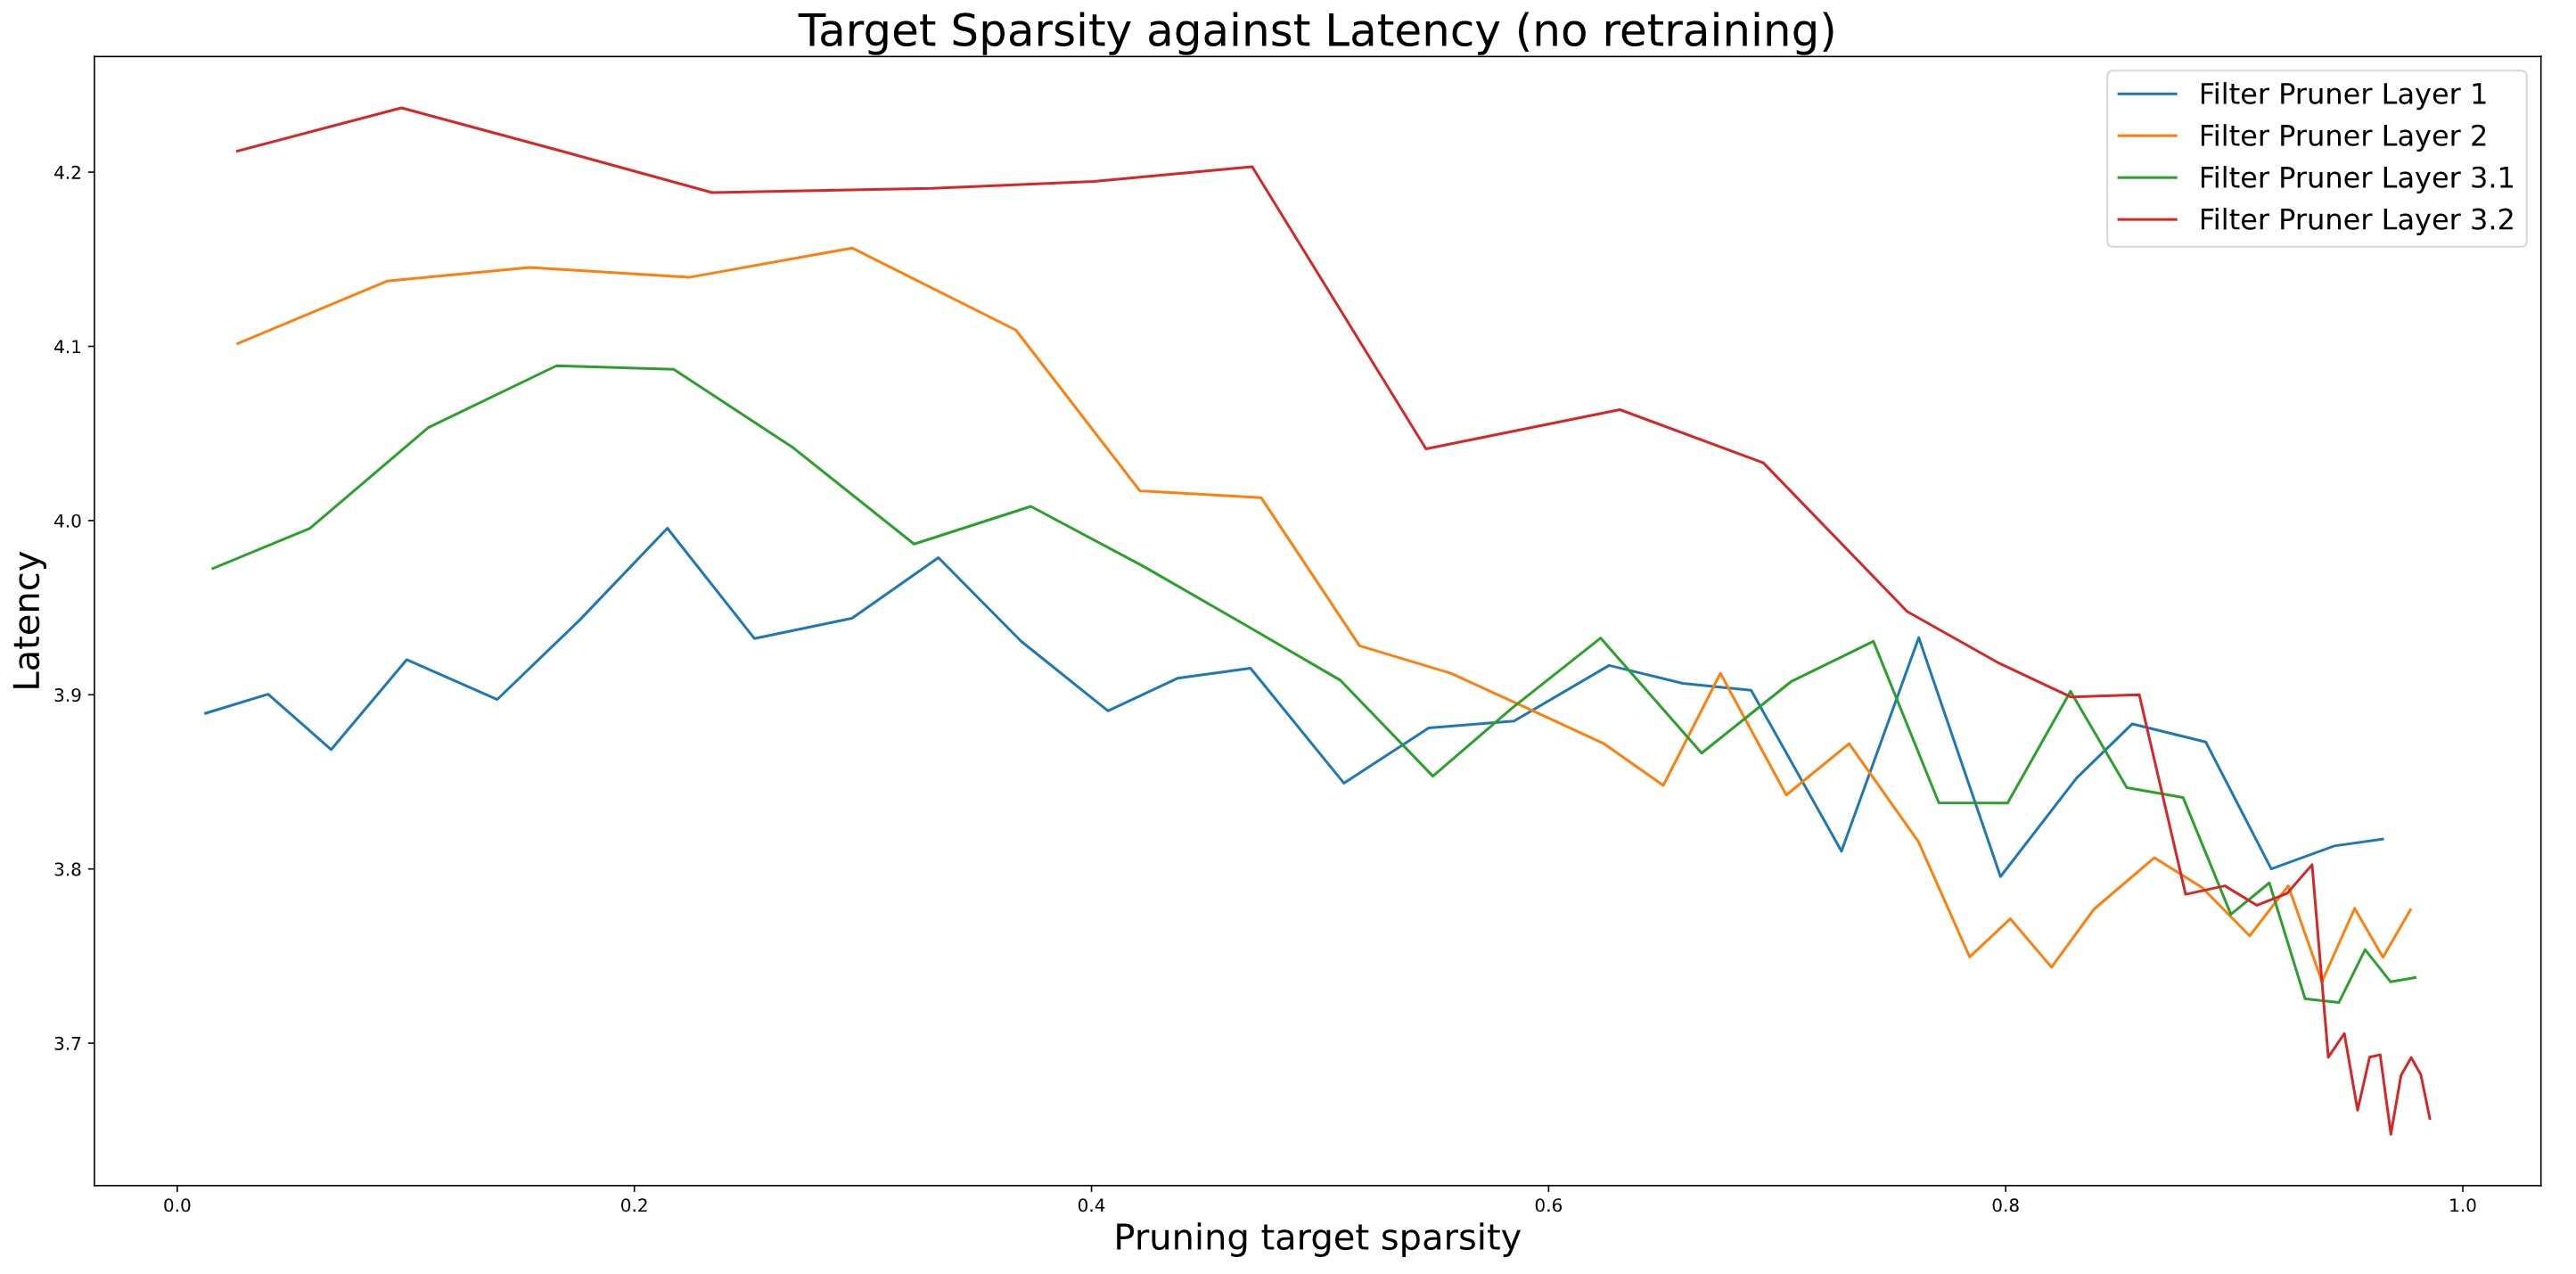
\includegraphics[width=1\textwidth]{TargetSparsityVsLatency_No_Retrain.jpg}
    \caption{Each pruner target sparsity plotted against mean Latency per bin.}
    \label{fig:fastPruneParamVSLatency}
\end{figure}

As discussed in section~\ref{sec:ex1} for this experiment we set the training epochs to 0 and set the target metric to minimize latency. 
During this phase of the experiment we gathered data to observe how pruning would affect latency, this was useful as an initial proof of concept.
This phase of the experiment was very time efficient, we were able to perform 1631 runs with around 18 hours of compute time; each run usually lasted between 24-55 seconds. 
Figure~\ref{fig:fastPruneParamVSLatency} shows the mean Latency computed by using equal width binning, where each bin represents parameter values inside each discretized 0.02 range between 0.0 and 1.0.
This chart does obfuscate any relationship between the parameters, however we can see how the filter pruner on Layer 3.2 (red) plots a more dramatic change in latency than the Pruner on Layer 1 (blue), this is also supported by computing the correlation between these values, see Table~\ref{tab:fastPruneCorrelations}, where `Filter Pruner Layer 3.2' has a strong negative correlation with Latency indicating that increasing the desired sparsity results in an increased tendency to observe a lower latency than `Filter Pruner Layer 1'.

\singlespacing
\begin{table}[H]
    \centering
    \begin{tabular}{@{}cp{26mm}p{26mm}p{26mm}p{26mm}@{}}
    \toprule
    \textbf{Metric}  & \textbf{Filter Pruner  Layer 1} & \textbf{Filter Pruner Layer 2} & \textbf{Filter Pruner Layer 3.1} & \textbf{Filter Pruner Layer 3.2} \\ \midrule
    \textbf{Latency} & $-0.80726$                        & $-0.40775$                      & $-0.11259$                         & $-0.552583$                         \\
    \textbf{Top1}    & $-0.152767$                       & $-0.104505$                     & $0.004462$                        & $-0.071923$                     \\ \bottomrule
    \end{tabular}
    \caption{Correlations between each target sparsity parameter and the metric being measured.}
    \label{tab:fastPruneCorrelations}
\end{table}
\doublespacing

We found that the degree to which we prune was not at all indicative of the resulting accuracy of the network before retraining, for example we observed networks with low desired sparsity across the board that had a much lower Top1 accuracy, than networks that were pruned with much higher targets (See models~\hyperref[sec:golden-sweep-523]{523},~\hyperref[sec:comfy-sweep-1007]{1007}).
It is interesting to note how weakly the pruning targets correlate with Top1 accuracy, this indicates that the relationship between accuracy and pruning is more complex than the naïve perception that pruning less has a smaller accuracy impact.
Observation of this weak correlation with Top1 prompted us to begin logging this initial set of metrics in addition to the metrics we logged as described in the Experimental Design Section~\ref{sec:metricsandparams} for experiments following this, we watched this data in the event that some pattern that might be indicative of how well a pruned network can recover accuracy before retraining has begun will emerge.

We observed a case where pruned networks that start with a Top1 accuracy of precisely $100 / n$ where $n$ is the number of classes would (according to our data) never recover any accuracy during retraining.
Due to the stochastic nature of retraining and the pruning algorithm we selected coupled with the fact that our methodology necessitated changing the pruning parameters each run we were unable to identify any other pattern or relationship between initial pruning metrics and the metrics of successful or high quality retrained networks from the data we gathered. 
Future investigation in this area should benchmark after every epoch with the intention of gaining some insight into how these metrics change over the retraining process, ideally we would aim to project how well a network might recover during the early stages of retraining, allowing us to make an informed decision on whether to abandon the model and try again or not.


\subsection{Experiment 2: Targeting Latency}\label{sec:Experiment2}

\singlespacing
\begin{table}[H]
    \centering
    \begin{tabular}{@{}cp{26mm}p{26mm}p{26mm}p{26mm}@{}}
    \toprule
    \textbf{Metric}  & \textbf{Filter Pruner  Layer 1} & \textbf{Filter Pruner Layer 2} & \textbf{Filter Pruner Layer 3.1} & \textbf{Filter Pruner Layer 3.2} \\ \midrule
    \textbf{Latency} & $-0.827473$                        & $-0.500734$                      & $-0.138894$                         & $-0.503688$                         \\
    \textbf{Top1}    & $-0.804794$                        & $-0.451589$                      & $-0.086224$                        & $-0.441157$                        \\ \bottomrule
    \end{tabular}
    \caption{Correlations between each target sparsity parameter and the metric being measured.}
    \label{tab:Ex2PruneCorrelations}
\end{table}
\doublespacing

As part of Objective~\hyperref[obj:AutoParams]{O6} we extended the first experiment and introduced 70 epochs of retraining to the system. 
At this stage we observed an interesting relationship between the retraining process and a further reduction in latency; the lowest latency run without retraining was $3.277$ms, out of the 256 successful runs with retraining in this experiment 12 were below the lowest latency from the first experiment.
This experiment managed to beat the best latency from the first experiment in 131 runs, however these 131 runs took approximately 36 hours of compute time compared to the (approximately) 4.5 hours it took the first experiment to achieve its best latency.
The lowest latency model (Model~\hyperref[sec:sec:unique-sweep-182]{182}) we recorded achieved an inference latency of $3.091$ms after retraining, this same model logged a latency of $3.529$ms before retraining, approximately 75\% of models in this experiment lost between $0.1$ms and $0.4$ms latency during retraining, the models that gained latency also tended to have a higher initial latency.
Despite the additional latency reduction as a result of retraining, the correlation (Table~\ref{tab:Ex2PruneCorrelations}) between each pruner and latency remains consistent with our initial observations from the first experiment (Table~\ref{tab:fastPruneCorrelations}), this lends some reliability to our results.


\begin{figure}[H]
    \centering
    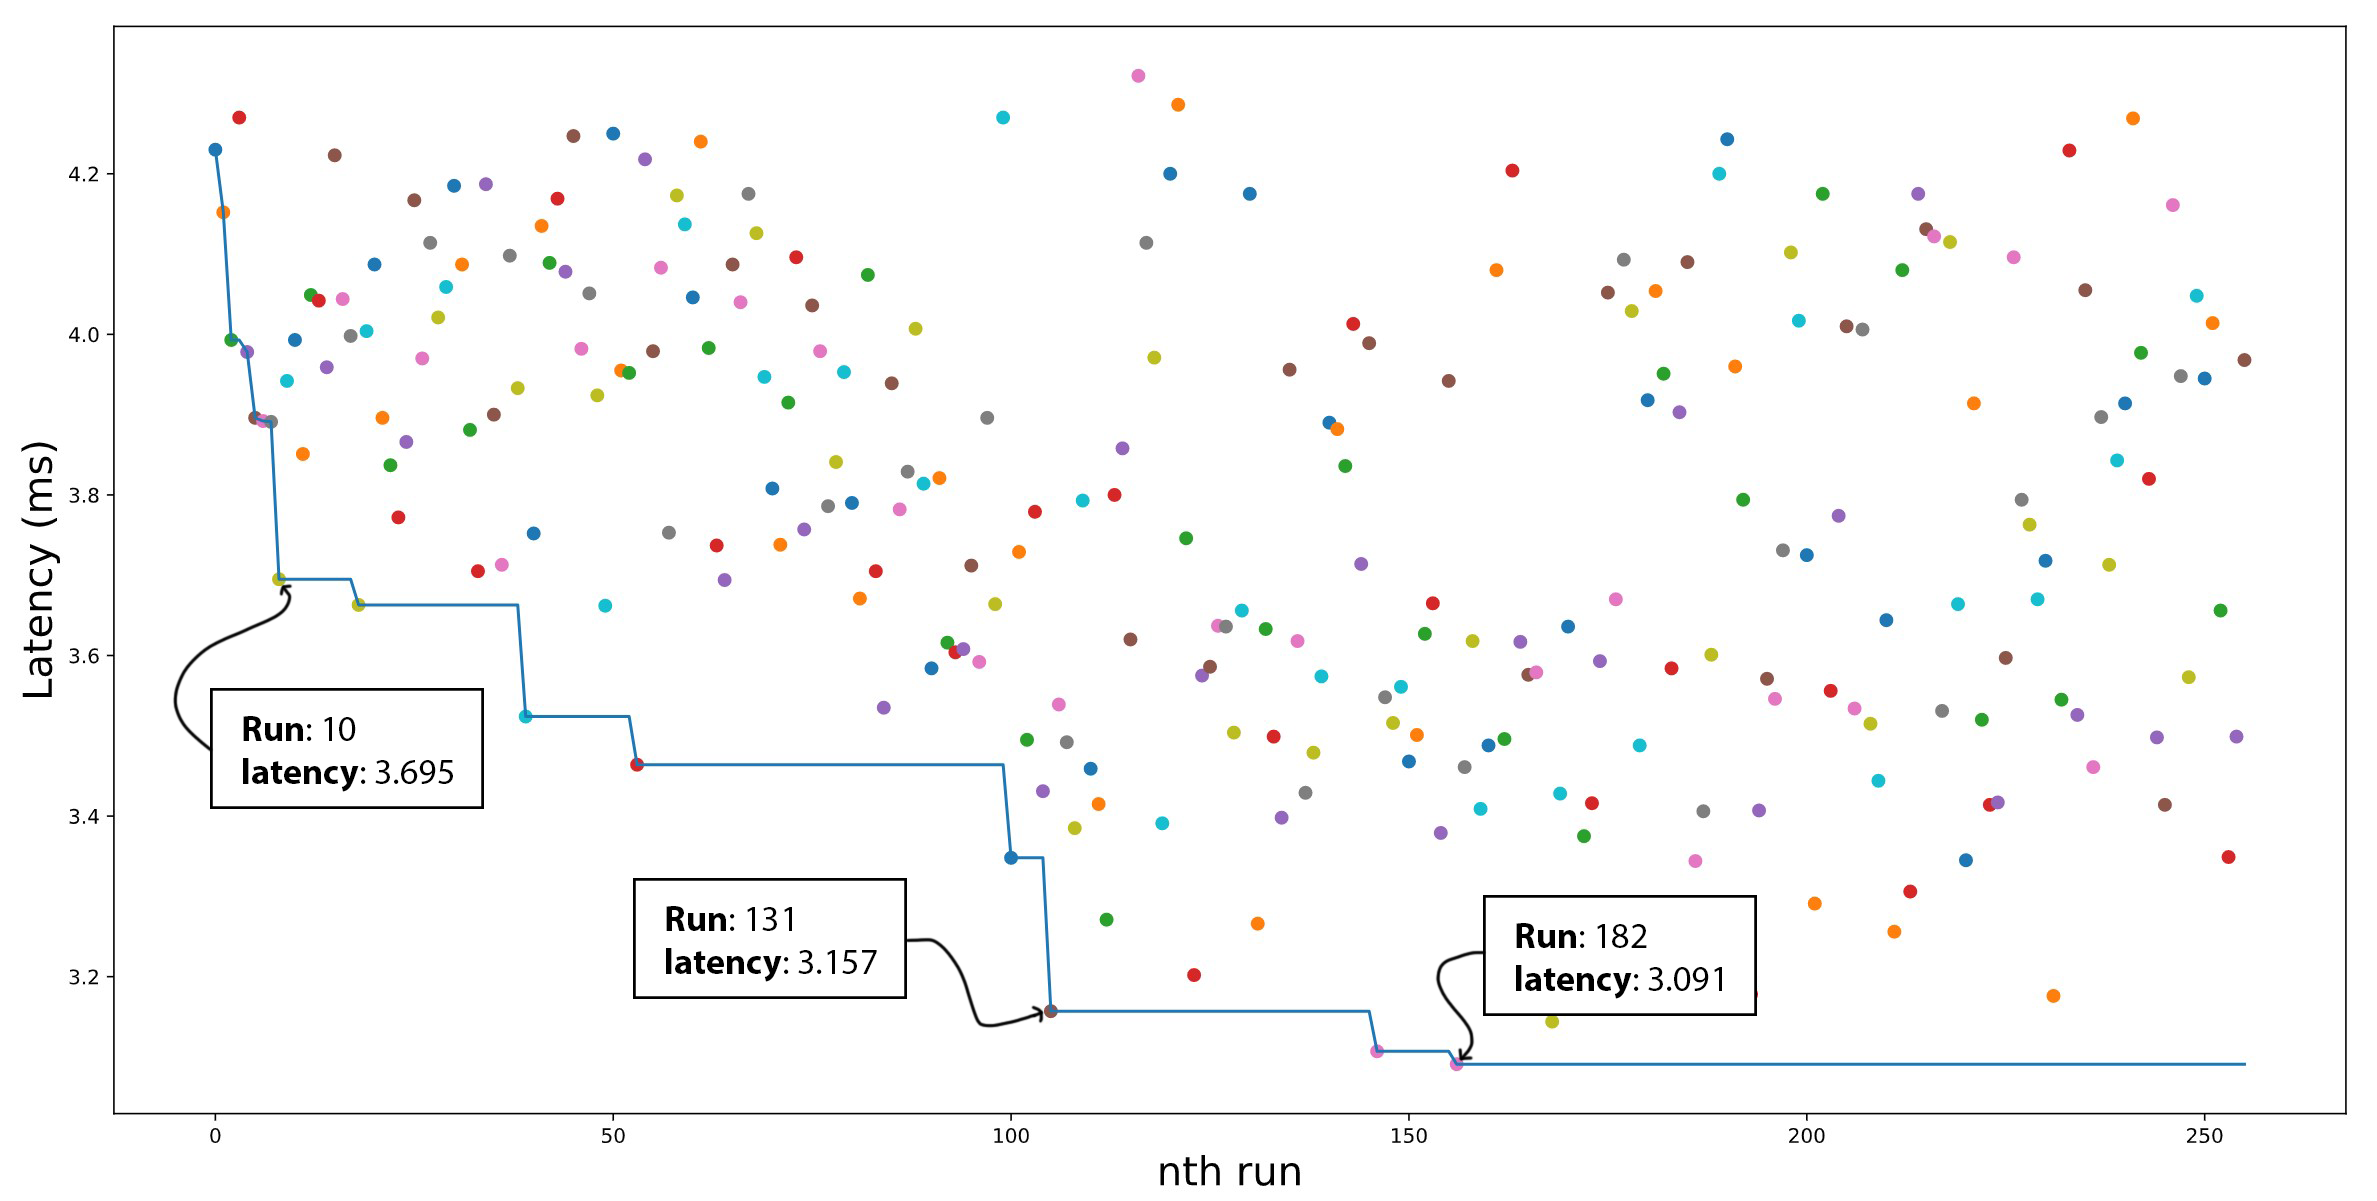
\includegraphics[width=\textwidth]{Ex2_Latency_over_runs_annotated.png}
    \caption{Experiment 2. Number of runs against Latency}
\end{figure}

\subsection{Experiment 3: Targeting Top1}

\singlespacing
\begin{table}[H]
    \centering
    \begin{tabular}{@{}cp{26mm}p{26mm}p{26mm}p{26mm}@{}}
    \toprule
    \textbf{Metric}  & \textbf{Filter Pruner  Layer 1} & \textbf{Filter Pruner Layer 2} & \textbf{Filter Pruner Layer 3.1} & \textbf{Filter Pruner Layer 3.2} \\ \midrule
    \textbf{Latency} & $-0.764499$                        & $-0.18715$                      & $-0.143377$                         & $-0.378644$                         \\
    \textbf{Top1}    & $-0.661244$                        & $-0.213514$                      & $-0.066348$                        & $-0.283732$                        \\ \bottomrule
    \end{tabular}
    \caption{Correlations between each target sparsity parameter and the metric being measured.}
    \label{tab:Ex3PruneCorrelations}
\end{table}
\doublespacing

In this experiment the focus is on Top1 accuracy, similarly to Experiment 2 we use 70 epochs for retraining, and a learning rate of 0.1. 
In table~\ref{fig:ex3Top1Rate} we see the Bayesian optimisation algorithm's effectiveness, after just 17 runs we find a Top1 of $88.52$ already very close to the global best Top1 of $88.77$ found after 147 runs in this experiment.
However the cost to latency is significant, only 5 runs had less than $3.5$ms latency, of those 5 only 1 had a Top1 below 86.5.
The quality of models produced was consistently higher in this experiment than when targeting latency, the mean Top1 was 87.2 and the median was 87.7, which when compared to the mean (85.3) and median (87.1) of Experiment 2 shows how important it is to account for Top1 accuracy when performing this kind of optimisation.
When we don't consider Top1 in our target metric we observed a 5x higher rate of ruined networks with accuracy that cannot be recovered by retraining.

\begin{figure}[H]
    \centering
    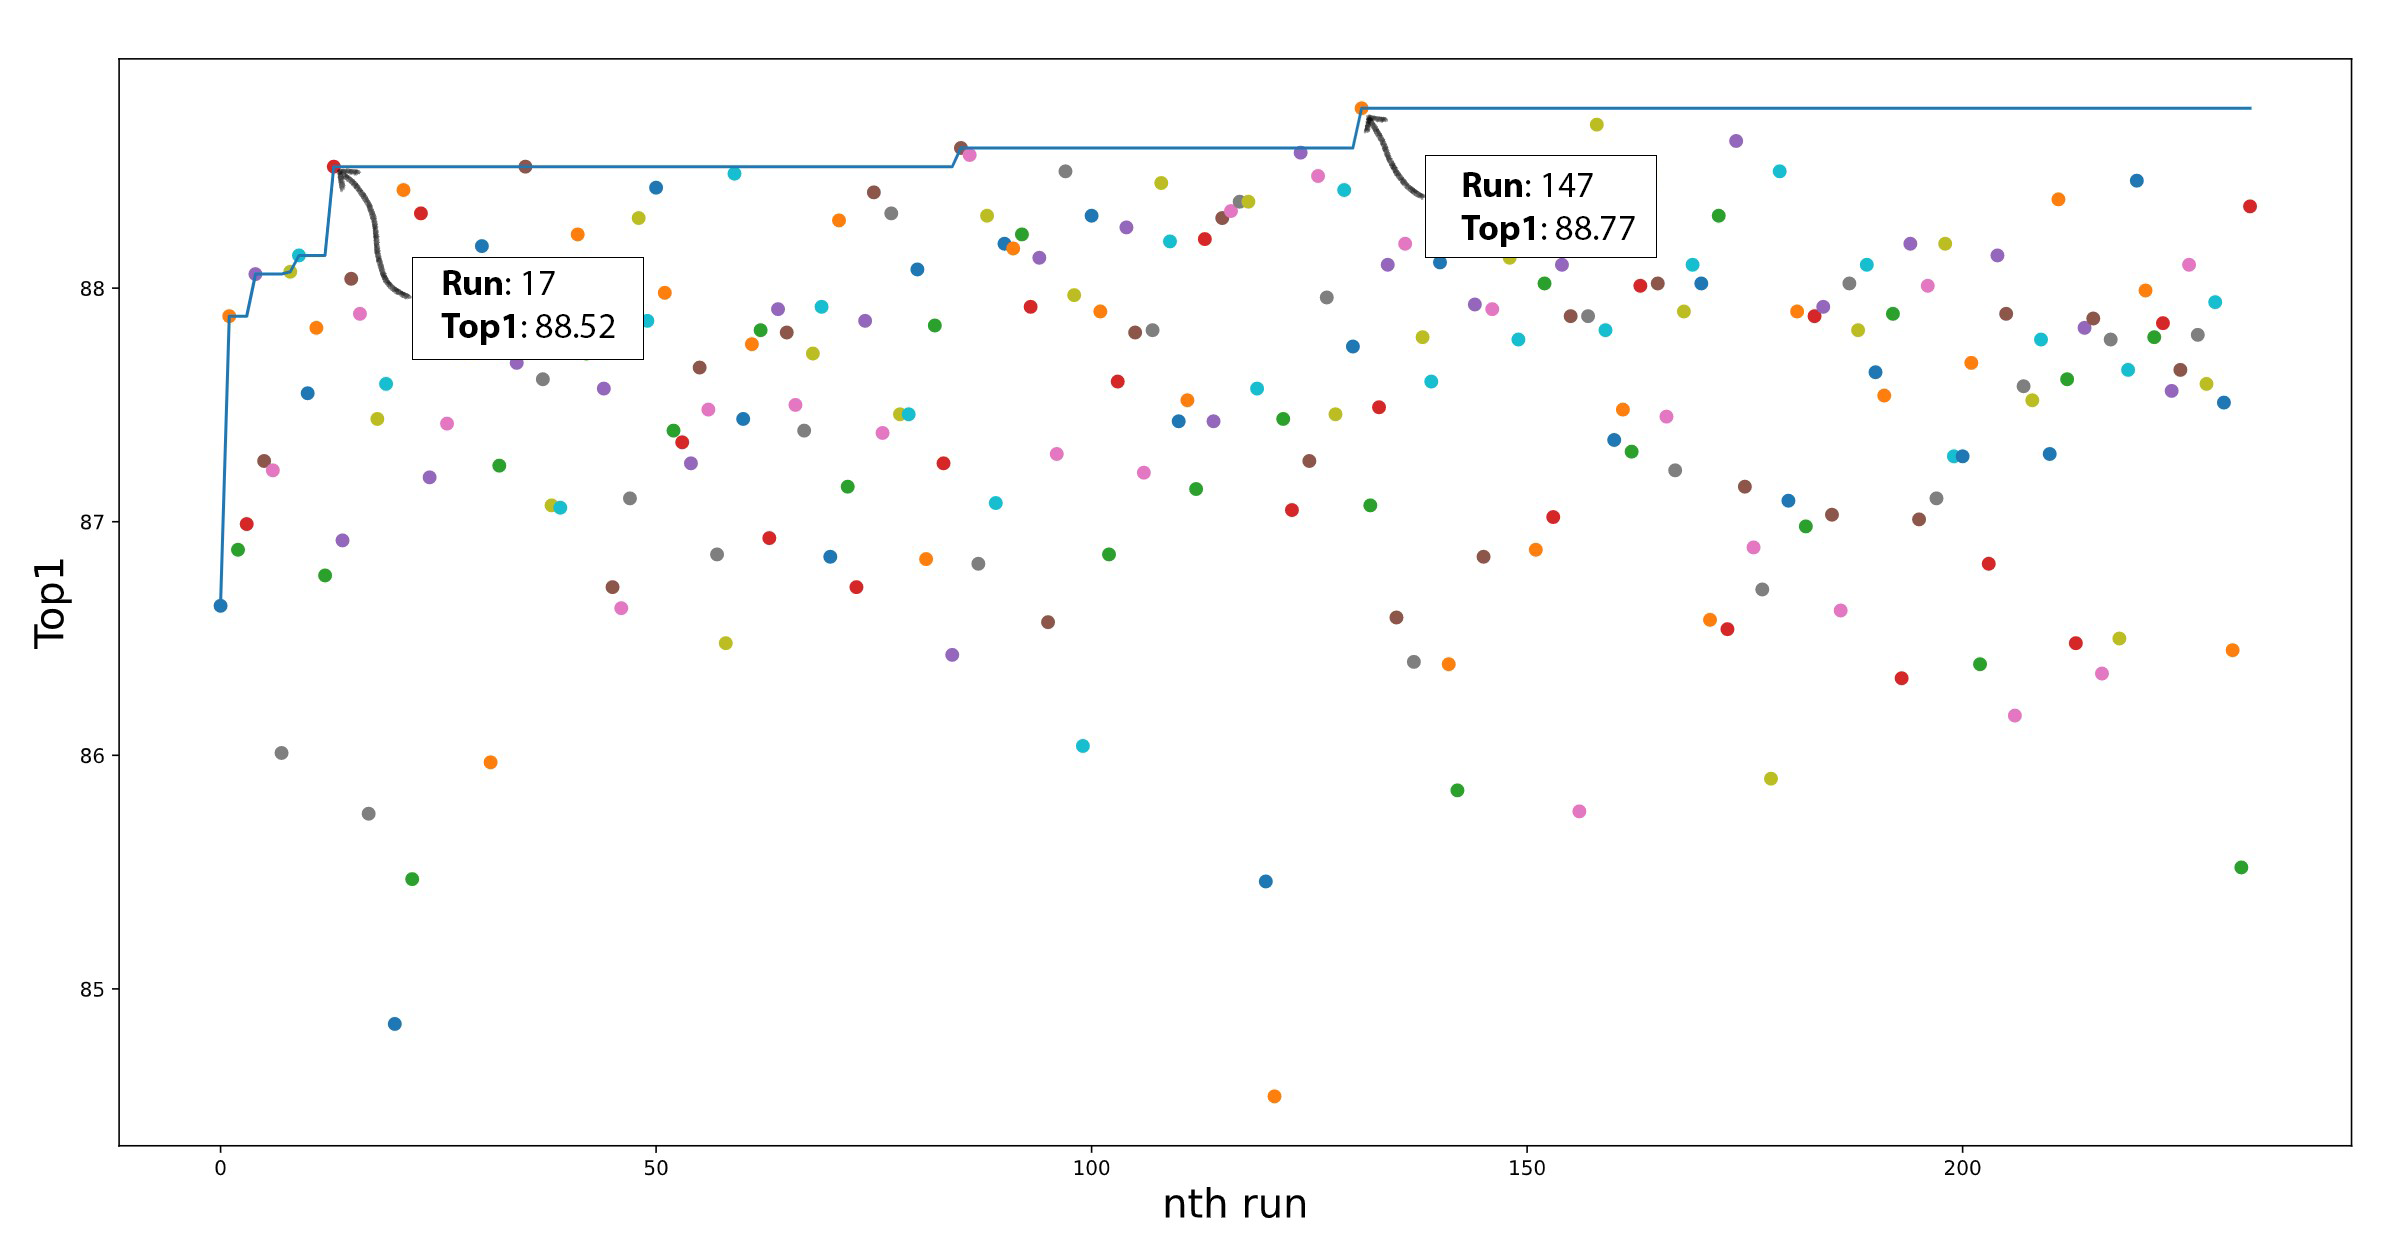
\includegraphics[width=\textwidth]{Ex3_scatterTop1runsAnnotated.png}
    \caption{Experiment 3. Number of runs to achieve best Top1 accuracy.}
    \label{fig:ex3Top1Rate}
\end{figure}

\subsection{Comparisons against baseline}

\begin{table}[H]
    \begin{tabular}{@{}lccp{25mm}p{23mm}p{28mm}@{}}
    \toprule
    \multicolumn{1}{c}{\textbf{Model}} & \textbf{Top1} & \textbf{Top5} & \textbf{Throughput (FPS)} & \textbf{Latency (ms)} & \textbf{Total Latency (ms)} \\ \midrule
    Baseline - no pruning              & 92.58         & 99.78         & 294.08                    & 4.375                 & 13.19                       \\
    Off the shelf - no retraining      & 11.19         & 51.02         & 303.98                    & 3.947                 & 12.89                       \\
    Off the shelf - retrained          &  87.72        & 99.47         & 305.27                    & 3.88                  & 12.95                           \\ \bottomrule
    \end{tabular}
    \caption{Baseline data, as gathered in Section~\ref{sec:baselineData}}
\end{table}




\textbf{Interesting observations}
\begin{itemize}
    \item The models that lost all predictive power due to overpruning were not the fastest, even when targeting only latency.
    \item The relationship between more pruning and lower latency is not as simple as you get a faster model with fewer tensors
    \item When targeting accuracy we found models with as low latency when targeting latency directly.
    \item When targeting latency we found models with as high accuracy as when targeting accuracy directly.
    \item Surprising to see that retraining reduces the latency also
\end{itemize}

\section{Further work}
\emph{
\begin{itemize}
	\item Suggested improvements for methodology
	\item Next steps
\end{itemize}
}

\begin{itemize}
    \item More datasets need to be tested
    \item More models should be used
    \item Layer selection should be automated
    \item how well does this system generalise?
    \item Further investigation should look at a relationship between higher accuracy models after only pruning and how they recover vs low accuracy models after pruning
    \item Why are there so few completely ruined networks before retraining compared to after retraining?
    \item Using this data to train a reinforcement learning dnn
\end{itemize}

Further investigation to identify which untrained pruned models will respond well to retraining (particularly with one-shot pruning methods) would be valuable because retraining is expensive and one-shot pruning is (comparatively) cheap.
This could help inform researchers or users of pruning systems weather they should try and prune again or 



\end{document}